% Generated by scripts/build_latex.py from docs/report/ch5_implementation.md: edit the Markdown, not this file.
\chapter{Coding and Implementation}\label{ch:5}

This chapter describes how the design was implemented: the main algorithms as pseudo-code (Section~\ref{sec:5.1}), the development environment (Section~\ref{sec:5.2}), the modules with their owners (Section~\ref{sec:5.3}), short extracts of the real code (Section~\ref{sec:5.4}) and the user interface (Section~\ref{sec:5.5}).

\FloatBarrier
\section{Algorithms / Steps}\label{sec:5.1}

Names in \code{code font} are the real functions and constants in the repository.

\begin{algorithm}[H]
  \caption{Orchestrator state machine (\code{Orchestrator.step}, \code{run\_\allowbreak{}until\_\allowbreak{}blocked})}\label{alg:5.1}
  \noindent\fcolorbox{codeframe}{codebg}{\begin{minipage}{\dimexpr\linewidth-2\fboxsep-2\fboxrule\relax}
  \linespread{1}\small
  \begin{algorithmic}
    \State \textbf{procedure} RUN\_UNTIL\_BLOCKED(ctx) \Comment{MAX\_STEPS = 50}
    \State \hspace*{1.50em}\textbf{repeat} MAX\_STEPS times
    \State \hspace*{3.00em}\textbf{if} ctx.state \ensuremath{\in} \{DONE, FAILED, NEEDS\_INPUT\} \textbf{then} \textbf{return} ctx
    \State \hspace*{3.00em}STEP(ctx)
    \State \hspace*{1.50em}TRANSITION(ctx, FAILED, ``stopped after MAX\_STEPS steps (possible loop)'')
    \Statex
    \State \textbf{procedure} STEP(ctx)
    \State \hspace*{1.50em}\textbf{try} (next, message) \ensuremath{\leftarrow} HANDLERS[ctx.state](ctx) \Comment{one handler per state}
    \State \hspace*{1.50em}\textbf{catch} error e: record e; next \ensuremath{\leftarrow} FAILED \Comment{never crash the caller}
    \State \hspace*{1.50em}TRANSITION(ctx, next, message)
    \Statex
    \State \textbf{procedure} TRANSITION(ctx, next, message)
    \State \hspace*{1.50em}append event(from, to, message, time) to ctx.history; ctx.state \ensuremath{\leftarrow} next
    \State \hspace*{1.50em}write state.json.tmp, then atomically replace state.json \Comment{\ensuremath{\leq} 3 retries on Windows locks}
    \State \hspace*{1.50em}\textbf{try} record run + event in SQLite (one transaction) \textbf{catch} \ensuremath{\rightarrow} log only
  \end{algorithmic}
  \end{minipage}}
\end{algorithm}

\begin{algorithm}[H]
  \caption{Requirement parsing and repair (\code{RequirementAgent.\allowbreak{}parse}, \code{repair}, \code{check\_\allowbreak{}sufficiency})}\label{alg:5.2}
  \noindent\fcolorbox{codeframe}{codebg}{\begin{minipage}{\dimexpr\linewidth-2\fboxsep-2\fboxrule\relax}
  \linespread{1}\small
  \begin{algorithmic}
    \State R \ensuremath{\leftarrow} LLM structured output for question q and format\_profile(P) \Comment{names, types, \% missing only}
    \State \hspace*{1.50em}(no LLM: R \ensuremath{\leftarrow} requirement\_from\_profile(q, P))
    \State \textbf{if} R.target is not a usable column of P (numeric / categorical / boolean, \textgreater{} 1 value)
    \State \hspace*{1.50em}\textbf{then} note the reason; R.target \ensuremath{\leftarrow} P.suggested\_target
    \State \textbf{if} task type implied by P for R.target \ensuremath{\neq} R.task\_type \textbf{then} note; R.task\_type \ensuremath{\leftarrow} implied type
    \State remove metrics of the wrong family; \textbf{if} none left \textbf{then} R.metrics \ensuremath{\leftarrow} TASK\_METRICS[task]
    \State missing \ensuremath{\leftarrow} rules (goal unclear? no target for a supervised task? confidence \textless{} 0.4?) \ensuremath{\cup} LLM review
    \State \textbf{if} missing \ensuremath{\neq} \ensuremath{\emptyset} \textbf{then} ask \ensuremath{\leq} 3 clarifying questions \ensuremath{\rightarrow} NEEDS\_INPUT (at most 2 rounds per run)
  \end{algorithmic}
  \end{minipage}}
\end{algorithm}

\begin{algorithm}[H]
  \caption{AutoML search, selection and single test evaluation (\code{AutoMLTrainer.run}, \code{tuner.tune})}\label{alg:5.3}
  \noindent\fcolorbox{codeframe}{codebg}{\begin{minipage}{\dimexpr\linewidth-2\fboxsep-2\fboxrule\relax}
  \linespread{1}\small
  \begin{algorithmic}
    \State (train, valid, test) \ensuremath{\leftarrow} SPLIT(D, 70/20/10); wrap test in Holdout; fit preprocessing on train
    \State \textbf{for} each candidate m in the plan (\ensuremath{\leq} budget.max\_candidates) \textbf{do}
    \State \hspace*{1.50em}\textbf{if} total time is used up \textbf{then} mark m ``skipped''; continue
    \State \hspace*{1.50em}study \ensuremath{\leftarrow} Optuna(TPE sampler(seed), median pruner)
    \State \hspace*{1.50em}\textbf{for} each trial (\ensuremath{\leq} n\_trials, \ensuremath{\leq} timeout per model) \textbf{do}
    \State \hspace*{3.00em}\ensuremath{\theta} \ensuremath{\leftarrow} sample(m.search\_space)
    \State \hspace*{3.00em}\textbf{if} \textbar{}train\textbar{} \ensuremath{\geq} 2000 \textbf{then} score on half the rows first; prune \textbf{if} below the median
    \State \hspace*{3.00em}score \ensuremath{\leftarrow} metric(fit(m, \ensuremath{\theta}, train), valid) \Comment{errors \ensuremath{\rightarrow} trial pruned, search continues}
    \State \hspace*{1.50em}refit best \ensuremath{\theta} on train; tune threshold \textbf{if} binary (Algorithm 5.4); record valid score, time, size
    \State mark constraint violations; best \ensuremath{\leftarrow} best valid score without violations
    \State model \ensuremath{\leftarrow} Pipeline(preprocessing, best) refitted on train \ensuremath{\cup} valid
    \State score model and a trivial baseline on Holdout.reveal(``final\_evaluation'') \Comment{the only test read}
  \end{algorithmic}
  \end{minipage}}
\end{algorithm}

\begin{algorithm}[H]
  \caption{Decision-threshold tuning (\code{evaluator.\allowbreak{}tune\_\allowbreak{}threshold})}\label{alg:5.4}
  \noindent\fcolorbox{codeframe}{codebg}{\begin{minipage}{\dimexpr\linewidth-2\fboxsep-2\fboxrule\relax}
  \linespread{1}\small
  \begin{algorithmic}
    \State (t*, s*) \ensuremath{\leftarrow} (0.5, M(y\_valid, p \ensuremath{\geq} 0.5))
    \State \textbf{for} t in 0.05, 0.06, \ldots{}, 0.95 \textbf{do} \Comment{91 cut-offs, validation split only}
    \State \hspace*{1.50em}s \ensuremath{\leftarrow} M(y\_valid, p \ensuremath{\geq} t); \textbf{if} s \textgreater{} s* \textbf{then} (t*, s*) \ensuremath{\leftarrow} (t, s) \Comment{ties keep 0.5}
    \State \textbf{return} t* \Comment{M \ensuremath{\in} \{F1, accuracy, balanced accuracy\}}
  \end{algorithmic}
  \end{minipage}}
\end{algorithm}

\begin{algorithm}[H]
  \caption{Verification and re-planning (\code{Verifier.verify}, \code{Orchestrator.\allowbreak{}\_\allowbreak{}handle\_\allowbreak{}verify})}\label{alg:5.5}
  \noindent\fcolorbox{codeframe}{codebg}{\begin{minipage}{\dimexpr\linewidth-2\fboxsep-2\fboxrule\relax}
  \linespread{1}\small
  \begin{algorithmic}
    \State checks \ensuremath{\leftarrow} metric targets met \ensuremath{\cdot} beats the baseline \ensuremath{\cdot} no constraint violated \ensuremath{\cdot} \ensuremath{\geq} 30 test rows \ensuremath{\cdot}
    \State \hspace*{3.38em}test accesses = [``final\_evaluation''] \ensuremath{\cdot} no leakage warning \ensuremath{\cdot} train \ensuremath{-} test gap \textless{} 0.15
    \State \textbf{if} all pass \textbf{then} next \ensuremath{\leftarrow} EXPLAIN
    \State \textbf{else} \textbf{if} not yet re-planned \textbf{then} next \ensuremath{\leftarrow} PLAN with the full budget and the checks' recommendations
    \State \textbf{else} next \ensuremath{\leftarrow} EXPLAIN, results flagged ``not verified'' \Comment{never FAILED for this reason}
  \end{algorithmic}
  \end{minipage}}
\end{algorithm}

\begin{algorithm}[H]
  \caption{Greedy counterfactual search (\code{recommender.\allowbreak{}counterfactual})}\label{alg:5.6}
  \noindent\fcolorbox{codeframe}{codebg}{\begin{minipage}{\dimexpr\linewidth-2\fboxsep-2\fboxrule\relax}
  \linespread{1}\small
  \begin{algorithmic}
    \State p \ensuremath{\leftarrow} f(x); \ensuremath{\Delta} \ensuremath{\leftarrow} []
    \State \textbf{repeat} at most 3 times \textbf{while} p \ensuremath{\geq} t
    \State \hspace*{1.50em}\textbf{try} every (column a \ensuremath{\in} actionable \ensuremath{\setminus} \ensuremath{\Delta}, observed value v \ensuremath{\neq} x[a]) in one batch
    \State \hspace*{1.50em}take the option with the lowest probability p\ensuremath{{}'}; stop \textbf{if} p\ensuremath{{}'} \ensuremath{\geq} p
    \State \hspace*{1.50em}x[a] \ensuremath{\leftarrow} v; \ensuremath{\Delta} \ensuremath{\leftarrow} \ensuremath{\Delta} \ensuremath{\cup} \{a\}; p \ensuremath{\leftarrow} p\ensuremath{{}'}
    \State \textbf{if} p \textless{} t \textbf{then} undo every change in \ensuremath{\Delta} that is not needed to stay below t \Comment{minimal set}
    \State \textbf{return} \ensuremath{\Delta}, probability before and after, success = (p \textless{} t)
  \end{algorithmic}
  \end{minipage}}
\end{algorithm}

\begin{algorithm}[H]
  \caption{Grounded insight generation (\code{InsightAgent.\allowbreak{}generate}, \code{unsupported\_\allowbreak{}numbers})}\label{alg:5.7}
  \noindent\fcolorbox{codeframe}{codebg}{\begin{minipage}{\dimexpr\linewidth-2\fboxsep-2\fboxrule\relax}
  \linespread{1}\small
  \begin{algorithmic}
    \State \textbf{if} no LLM \textbf{then} \textbf{return} TEMPLATE(facts) \Comment{complete and itself grounded}
    \State allowed \ensuremath{\leftarrow} every number in the facts (also inside strings)
    \State \textbf{for} attempt = 1, 2 \textbf{do}
    \State \hspace*{1.50em}draft \ensuremath{\leftarrow} LLM(facts, feedback)
    \State \hspace*{1.50em}bad \ensuremath{\leftarrow} numbers in draft not in \{0..10, 100\} and not matching a fact (\ensuremath{\pm}1\%, rounding, \ensuremath{\times}100 for \%)
    \State \hspace*{1.50em}\textbf{if} bad = \ensuremath{\emptyset} \textbf{then} \textbf{return} draft
    \State \hspace*{1.50em}feedback \ensuremath{\leftarrow} ``numbers not in the facts: '' + bad
    \State \textbf{return} TEMPLATE(facts) with the failed grounding result
  \end{algorithmic}
  \end{minipage}}
\end{algorithm}

\begin{algorithm}[H]
  \caption{Sandboxed execution of LLM-written code (\code{sandbox.check\_\allowbreak{}code}, \code{run\_\allowbreak{}code})}\label{alg:5.8}
  \noindent\fcolorbox{codeframe}{codebg}{\begin{minipage}{\dimexpr\linewidth-2\fboxsep-2\fboxrule\relax}
  \linespread{1}\small
  \begin{algorithmic}
    \State reject code \textgreater{} 20 000 characters or with a syntax error
    \State \textbf{for} each AST node: import outside \{pandas, numpy, math, statistics, datetime, json, re\},
    \State \hspace*{1.50em}blocked name (open, eval, exec, \_\_import\_\_, getattr, os, sys, \ldots{}), private attribute,
    \State \hspace*{1.50em}I/O attribute (read\_*, to\_csv, \ldots{}) or other blocked attribute (query, load, \ldots{}) \ensuremath{\rightarrow} problem
    \State \textbf{if} problems \textbf{then} \textbf{return} ``Blocked by the sandbox'' (nothing runs)
    \State run ``python -I sandbox\_runner.py'' in a temporary folder with restricted built-ins,
    \State \hspace*{1.50em}a guarded \_\_import\_\_ and an environment without secrets; kill after the timeout (20 s)
    \State \textbf{return} stdout (\ensuremath{\leq} 20 KB) and result (\ensuremath{\leq} 200 rows)
  \end{algorithmic}
  \end{minipage}}
\end{algorithm}

\FloatBarrier
\section{Software and Hardware for Development}\label{sec:5.2}

The runtime libraries are those of Table~\ref{tab:4.5}. Table~\ref{tab:5.1} lists the additional development tools and Table~\ref{tab:5.2} the hardware.

\begin{table}[H]
\centering
\linespread{1}\small
\setlength{\tabcolsep}{4pt}
\caption{Development tools}\label{tab:5.1}
\begin{tabular}{|>{\raggedright\arraybackslash\hspace{0pt}}p{\dimexpr 0.2675\linewidth-2\tabcolsep-2\arrayrulewidth\relax}|>{\raggedright\arraybackslash\hspace{0pt}}p{\dimexpr 0.2254\linewidth-2\tabcolsep-2\arrayrulewidth\relax}|>{\raggedright\arraybackslash\hspace{0pt}}p{\dimexpr 0.5071\linewidth-2\tabcolsep-2\arrayrulewidth\relax}|}
\hline
\rowcolor{tableheader}\textbf{Tool} & \textbf{Version} & \textbf{Use} \\
\hline
Python \code{venv} + pip & Python 3.12.0 & Isolated environment with pinned dependencies (\code{requirements.txt}) \\ \hline
pytest, pytest-cov, httpx2 & 9.1.1, 7.1.0, 2.13.1 & Automated tests, coverage, API test client \\ \hline
ruff & 0.16.10 & Linting \\ \hline
Playwright (Chromium) & 1.63.0 & Automated UI screenshots \\ \hline
Git & --- & Version control, one commit per increment \\ \hline
PowerShell & Windows PowerShell & Start scripts (\code{run\_\allowbreak{}api.ps1}, \code{run\_\allowbreak{}ui.ps1}, \code{run\_\allowbreak{}all.ps1}) \\ \hline
Claude Code & --- & AI coding assistant for code generation and refactoring \\ \hline
\end{tabular}
\end{table}

An AI coding assistant (Claude Code) was used to help generate and refactor code; all design decisions, integration, testing and evaluation were carried out and verified by the team.

\begin{table}[H]
\centering
\linespread{1}\small
\setlength{\tabcolsep}{4pt}
\caption{Development hardware}\label{tab:5.2}
\begin{tabular}{|>{\raggedright\arraybackslash\hspace{0pt}}p{\dimexpr 0.2571\linewidth-2\tabcolsep-2\arrayrulewidth\relax}|>{\raggedright\arraybackslash\hspace{0pt}}p{\dimexpr 0.7429\linewidth-2\tabcolsep-2\arrayrulewidth\relax}|}
\hline
\rowcolor{tableheader}\textbf{Item} & \textbf{Specification} \\
\hline
Development machine & ASUS TUF Gaming F15 (FX506HE) laptop, used for development, testing, the evaluation and this report \\ \hline
Processor & 11th Gen Intel Core i7-11800H, 2.30 GHz, 8 cores / 16 logical processors \\ \hline
Memory & 16 GB RAM \\ \hline
Storage & 1 TB NVMe SSD (WD PC SN560) \\ \hline
GPU & NVIDIA GeForce RTX 3050 Ti Laptop GPU (4 GB) --- not used by IDSS, which trains on the CPU \\ \hline
Operating system & Windows 11 Home Single Language, 64-bit \\ \hline
Network & Only for package installation and optional LLM calls \\ \hline
\end{tabular}
\end{table}

The evaluation of Chapter~\ref{ch:7} ran on this machine (\code{scripts/\allowbreak{}evaluate.\allowbreak{}py} records Windows 11 and 16 logical CPUs). The minimum hardware for running IDSS is given in Table~\ref{tab:4.4}.

\FloatBarrier
\section{Modules in Project}\label{sec:5.3}

\begingroup
\linespread{1}\small
\setlength{\tabcolsep}{4pt}
\begin{longtable}{|>{\raggedright\arraybackslash\hspace{0pt}}p{\dimexpr 0.0733\linewidth-2\tabcolsep-2\arrayrulewidth\relax}|>{\raggedright\arraybackslash\hspace{0pt}}p{\dimexpr 0.2628\linewidth-2\tabcolsep-2\arrayrulewidth\relax}|>{\raggedright\arraybackslash\hspace{0pt}}p{\dimexpr 0.3935\linewidth-2\tabcolsep-2\arrayrulewidth\relax}|>{\raggedright\arraybackslash\hspace{0pt}}p{\dimexpr 0.2704\linewidth-2\tabcolsep-2\arrayrulewidth\relax}|}
\caption{Modules and responsibilities}\label{tab:5.3}\\
\hline
\rowcolor{tableheader}\textbf{No.} & \textbf{Module} & \textbf{Main files} & \textbf{Member responsible} \\
\hline
\endfirsthead
\hline
\rowcolor{tableheader}\textbf{No.} & \textbf{Module} & \textbf{Main files} & \textbf{Member responsible} \\
\endhead
1 & Foundation & \code{configs/\allowbreak{}settings.\allowbreak{}py}, \code{idss/\allowbreak{}core/} & Raj Vishwas Patil, Chaitany Rajesh Naval \\ \hline
2 & Data module & \code{idss/\allowbreak{}ml/\allowbreak{}data\_\allowbreak{}loader.\allowbreak{}py}, \code{profiler.py}, \code{preprocess.py}, \code{agents/\allowbreak{}data\_\allowbreak{}agent.\allowbreak{}py} & Bhavesh Vinod Patil \\ \hline
3 & Requirement Agent and Orchestrator & \code{agents/\allowbreak{}requirement\_\allowbreak{}agent.\allowbreak{}py}, \code{agents/\allowbreak{}manager.py} & Raj Vishwas Patil, Chaitany Rajesh Naval \\ \hline
4 & AutoML engine and Model Agent & \code{idss/\allowbreak{}ml/\allowbreak{}model\_\allowbreak{}zoo.\allowbreak{}py}, \code{tuner.py}, \code{evaluator.py}, \code{trainer.py}, \code{agents/\allowbreak{}model\_\allowbreak{}agent.\allowbreak{}py} & Bhavesh Vinod Patil, Raj Vishwas Patil \\ \hline
5 & Knowledge base & \code{idss/\allowbreak{}knowledge/}, \code{data/\allowbreak{}knowledge/}, \code{agents/\allowbreak{}knowledge\_\allowbreak{}agent.\allowbreak{}py} & Raj Vishwas Patil \\ \hline
6 & Verifier & \code{agents/\allowbreak{}verifier.py} & Bhavesh Vinod Patil \\ \hline
7 & Sandbox and Analysis Agent & \code{idss/\allowbreak{}execution/}, \code{agents/\allowbreak{}analysis\_\allowbreak{}agent.\allowbreak{}py} & Chaitany Rajesh Naval \\ \hline
8 & Decision layer & \code{idss/\allowbreak{}ml/\allowbreak{}explain.py}, \code{idss/\allowbreak{}decision/\allowbreak{}what\_\allowbreak{}if.\allowbreak{}py}, \code{recommender.py} & Bhavesh Vinod Patil \\ \hline
9 & Insight Agent and reports & \code{agents/\allowbreak{}insight\_\allowbreak{}agent.\allowbreak{}py}, \code{idss/\allowbreak{}decision/\allowbreak{}report\_\allowbreak{}builder.\allowbreak{}py} & Raj Vishwas Patil, Varun Darshan Patil \\ \hline
10 & Storage and REST API & \code{idss/\allowbreak{}storage/}, \code{api/} & Chaitany Rajesh Naval \\ \hline
11 & Streamlit UI & \code{ui/} & Varun Darshan Patil \\ \hline
12 & Evaluation and tooling & \code{scripts/} & Bhavesh Vinod Patil, Varun Darshan Patil \\ \hline
\end{longtable}
\endgroup

The member column follows the roles of Table~\ref{tab:3.4} and the planned allocation of Table~\ref{tab:3.5}; testing, review and integration of every module were shared by the whole team.

\textbf{1. Foundation.} Typed settings from \code{.env} (keys as secret strings, never logged); one logger (loguru, rotating at 10 MB); the only LLM client --- OpenAI-compatible, 60 s default timeout, at most 3 retries with exponential backoff, and \code{chat\_\allowbreak{}structured()}, which validates replies against a Pydantic model and feeds errors back for a retry; the shared Pydantic schemas; and eleven prompt templates with \code{\#\# system} / \code{\#\# user} sections.

\textbf{2. Data module.} Loads CSV (delimiter and encoding detection), Excel, JSON / JSON lines and Parquet; profiles semantic types (numeric, categorical, boolean, datetime, id, text), missing values, the suggested target and task, and warns about leakage (correlation with the target \ensuremath{\geq} 0.98) and imbalance; cleans the data, splits it 70/20/10 and fits a preprocessor (imputation, scaling, one-hot encoding capped at 20 categories). The Data Agent asks the LLM only for a summary of aggregates. \textit{Output:} profile, Parquet splits and \code{preprocessor.\allowbreak{}joblib}.

\textbf{3. Requirement Agent and Orchestrator.} Relevance, parsing, repair and clarifying questions (Algorithm~\ref{alg:5.2}), and the 13-state \code{RunState} machine (Algorithm~\ref{alg:5.1}) with \code{start}, \code{step}, \code{run\_\allowbreak{}until\_\allowbreak{}blocked}, \code{provide\_\allowbreak{}answer}, \code{resume}, \code{abort}, \code{ask} and \code{what\_\allowbreak{}if}. \textit{Output:} \code{RunContext} in \code{workspace/\allowbreak{}runs/\allowbreak{}\textless{}run\_\allowbreak{}id\textgreater{}/\allowbreak{}state.\allowbreak{}json}, mirrored to SQLite.

\textbf{4. AutoML engine and Model Agent.} The model zoo (Table~\ref{tab:5.4}) is the only source of trainable models; each candidate has a \code{build()} function and an Optuna search space, and class weighting switches on when the minority class is below 20\%. Time-series features use only earlier rows. The evaluator holds 19 metrics with their family and direction and measures training time, inference time per row and model size. The Model Agent lets the LLM rank zoo names only (unknown names dropped, requested models first, defaults filling the rest) and parses constraints such as ``inference under 5 ms'' into the plan. Budgets: \textit{fast} 3 models \ensuremath{\times} 15 trials (60 s each, 180 s total); \textit{full} 6 \ensuremath{\times} 40 (180 s each, 1,080 s total). \textit{Output:} \code{TrainingResult}, \code{best\_\allowbreak{}model.joblib}, leaderboard, metrics and test predictions.

\begin{table}[H]
\centering
\linespread{1}\small
\setlength{\tabcolsep}{4pt}
\caption{Model zoo and baselines}\label{tab:5.4}
\begin{tabular}{|>{\raggedright\arraybackslash\hspace{0pt}}p{\dimexpr 0.2698\linewidth-2\tabcolsep-2\arrayrulewidth\relax}|>{\raggedright\arraybackslash\hspace{0pt}}p{\dimexpr 0.5046\linewidth-2\tabcolsep-2\arrayrulewidth\relax}|>{\raggedright\arraybackslash\hspace{0pt}}p{\dimexpr 0.2256\linewidth-2\tabcolsep-2\arrayrulewidth\relax}|}
\hline
\rowcolor{tableheader}\textbf{Task} & \textbf{Candidate models} & \textbf{Baseline (test split)} \\
\hline
Classification & logistic regression, random forest, extra trees, XGBoost, LightGBM, histogram gradient boosting & Majority class \\ \hline
Regression & ridge, random forest, extra trees, XGBoost, LightGBM, histogram gradient boosting & Mean of the target \\ \hline
Time-series forecasting & LightGBM, XGBoost, ridge on lag / rolling / calendar features & Seasonal naive \\ \hline
Clustering & k-means, Gaussian mixture (several EM starts), agglomerative & Random assignment \\ \hline
\end{tabular}
\end{table}

\textbf{5. Knowledge base.} Ten notes in \code{data/\allowbreak{}knowledge/} (churn retention, class imbalance, clustering, explainability, feature leakage, model selection by data size, pricing and demand, regression, tabular classification, time series) are chunked (\ensuremath{\approx} 500 characters, 80 overlap), indexed with TF-IDF, cached and rebuilt when their content changes; retrieval returns 4 passages, at most 2 per note, which the Knowledge Agent condenses into a brief.

\textbf{6. Verifier.} Seven independent checks (Algorithm~\ref{alg:5.5}) with a fixed recommendation for each failure; an optional LLM review adds concerns but never changes the pass / fail decision.

\textbf{7. Sandbox and Analysis Agent.} The static guard and child-process runner of Algorithm~\ref{alg:5.8}; the Analysis Agent sends only column names and types to the LLM and asks it to repair failing code once.

\textbf{8. Decision layer.} \code{ModelExplainer} uses SHAP (tree or linear explainer, \ensuremath{\leq} 500 training rows) or permutation importance and maps values back to original columns; it also builds cluster profiles and a recursive forecast with a \ensuremath{\pm}1.96 \ensuremath{\times} validation-RMSE band. \code{what\_\allowbreak{}if.py} simulates records and segments with validated changes (value, set, add, pct) and structured filters, never evaluated strings. \code{recommender.py} infers actionable columns, builds risk tiers (High \ensuremath{\geq} max(threshold, 70th percentile), Medium \ensuremath{\geq} threshold, Low below), runs counterfactuals (Algorithm~\ref{alg:5.6}) on the 20 riskiest records and computes \ensuremath{\pm}10\% lever effects for regression; every recommendation carries its evidence.

\textbf{9. Insight Agent and reports.} \code{build\_\allowbreak{}facts()} is the only LLM input; the grounding check (Algorithm~\ref{alg:5.7}) guards the brief, with \code{template\_\allowbreak{}insight()} as fallback. \code{report\_\allowbreak{}builder.py} renders one block list as \code{report.pdf} (reportlab) and \code{report.md}.

\textbf{10. Storage and REST API.} SQLAlchemy models and a repository over SQLite; a FastAPI application with 17 endpoints (Table~\ref{tab:5.5}), errors as \code{\{error, detail\}}, \code{409 not\_\allowbreak{}ready} for results not yet computed, and one background RunWorker that answers \code{409 busy} to a second training request. Runs left unfinished by a previous process are marked FAILED at start-up.

\begingroup
\linespread{1}\small
\setlength{\tabcolsep}{4pt}
\begin{longtable}{|>{\raggedright\arraybackslash\hspace{0pt}}p{\dimexpr 0.1280\linewidth-2\tabcolsep-2\arrayrulewidth\relax}|>{\raggedright\arraybackslash\hspace{0pt}}p{\dimexpr 0.4590\linewidth-2\tabcolsep-2\arrayrulewidth\relax}|>{\raggedright\arraybackslash\hspace{0pt}}p{\dimexpr 0.4130\linewidth-2\tabcolsep-2\arrayrulewidth\relax}|}
\caption{REST API endpoints}\label{tab:5.5}\\
\hline
\rowcolor{tableheader}\textbf{Method} & \textbf{Path} & \textbf{Purpose} \\
\hline
\endfirsthead
\hline
\rowcolor{tableheader}\textbf{Method} & \textbf{Path} & \textbf{Purpose} \\
\endhead
GET & \code{/health} & Status, LLM configured (yes / no), version \\ \hline
POST, GET & \code{/datasets} & Upload a file (\ensuremath{\leq} 50 MB) with its profile; list datasets \\ \hline
GET & \code{/datasets/\allowbreak{}\{id\}/\allowbreak{}profile} & Profile of one dataset \\ \hline
POST, GET & \code{/runs} & Start a run (\code{202} + run id); list runs \\ \hline
GET & \code{/runs/\allowbreak{}\{id\}} & State, progress, events, metrics, verification, questions \\ \hline
POST & \code{/runs/\allowbreak{}\{id\}/\allowbreak{}answer} & Answer clarifying questions \\ \hline
GET & \code{/runs/\allowbreak{}\{id\}/\allowbreak{}leaderboard}, \code{/explanations}, \code{/recommendations}, \code{/insight} & Results of a finished run \\ \hline
POST & \code{/runs/\allowbreak{}\{id\}/\allowbreak{}what-if} & Record or segment simulation \\ \hline
POST & \code{/runs/\allowbreak{}\{id\}/\allowbreak{}ask} & Ask Your Data (\code{503} without an LLM) \\ \hline
GET & \code{/runs/\allowbreak{}\{id\}/\allowbreak{}report.\allowbreak{}pdf}, \code{/report.md}, \code{/charts/\allowbreak{}\{name\}} & Reports and charts (names and paths checked) \\ \hline
\end{longtable}
\endgroup

\textbf{11. Streamlit UI.} \code{ui/\allowbreak{}app.py} registers eight pages; \code{IDSSClient} is the UI's only route to the backend and turns connection errors into ``Backend not running -- start scripts/run\_api.ps1''; shared components provide the page shell, KPI cards, zebra tables, risk-tier chips, the pipeline stepper and Plotly charts. The Run Monitor polls every 2 s.

\textbf{12. Evaluation and tooling.} \code{make\_\allowbreak{}samples.py} (the five datasets), \code{evaluate.py} (Chapter~\ref{ch:7}), \code{benchmark\_\allowbreak{}step4.py}, the demo scripts, \code{make\_\allowbreak{}diagrams.py} (the diagrams in this report), \code{make\_\allowbreak{}screenshots.\allowbreak{}py} (Section~\ref{sec:5.5}) and \code{count\_\allowbreak{}loc.py} (Section~\ref{sec:3.3.2}).

\FloatBarrier
\section{Important Code Extracts}\label{sec:5.4}

The extracts below are copied from the repository (docstrings partly omitted). They enforce the main design rules.

\begin{lstlisting}[caption={One step of the state machine --- failures end the run cleanly (\code{idss/\allowbreak{}agents/\allowbreak{}manager.\allowbreak{}py})},label={lst:5.1}]
    def step(self, run_id: str | None = None) -> RunState:
        ctx = self._get(run_id)
        if ctx.state in BLOCKED_STATES:
            return ctx.state
        state = ctx.state
        try:
            next_state, message = self._handlers[state](ctx)
        # any failure ends the run cleanly instead of crashing the caller
        except Exception as exc:
            logger.exception("Run {} failed in state {}.", ctx.run_id, state)
            message = f"{state} failed: {type(exc).__name__}: {exc}"
            ctx.errors.append(message)
            ctx.message = f"Sorry, the run stopped during the {state.lower()}
                stage: {exc}"
            next_state = RunState.FAILED
        self._transition(ctx, next_state, message)
        return next_state
\end{lstlisting}

\begin{lstlisting}[caption={The audited test split (\code{idss/\allowbreak{}ml/\allowbreak{}trainer.py})},label={lst:5.2}]
class Holdout:
    """The test split. Reading it is logged so tests and the Verifier can
        prove it was used only once."""

    def __init__(self, frame: pd.DataFrame) -> None:
        self._frame = frame
        self.access_log: list[str] = []

    def __len__(self) -> int:
        return len(self._frame)

    def reveal(self, purpose: str) -> pd.DataFrame:
        self.access_log.append(purpose)
        logger.info("Test split accessed for: {}.", purpose)
        return self._frame
\end{lstlisting}

\begin{lstlisting}[caption={Decision-threshold search (\code{idss/\allowbreak{}ml/\allowbreak{}evaluator.\allowbreak{}py}, inside \code{tune\_\allowbreak{}threshold})},label={lst:5.3}]
    default_score = score(DEFAULT_THRESHOLD)
    best_threshold, best_score = DEFAULT_THRESHOLD, default_score
    for threshold in THRESHOLD_GRID:
        value = score(float(threshold))
        if value is not None and (best_score is None or value > best_score +
            1e-12):
            best_threshold, best_score = float(threshold), value
    return best_threshold, best_score, default_score
\end{lstlisting}

\begin{lstlisting}[caption={Static guard of the sandbox (\code{idss/\allowbreak{}execution/\allowbreak{}sandbox.\allowbreak{}py}, inside \code{check\_\allowbreak{}code})},label={lst:5.4}]
    for node in ast.walk(tree):
        if isinstance(node, ast.Import):
            problems += [f"import of '{a.name}' is not allowed" for a in
                node.names if not module_allowed(a.name)]
        elif isinstance(node, ast.ImportFrom):
            module = node.module or ""
            if node.level or not module_allowed(module):
                problems.append(f"import from '{module or '.'}' is not
                    allowed")
            problems += [f"importing '{a.name}' is not allowed" for a in
                node.names if _blocked_member(a.name)]
        elif isinstance(node, ast.Name) and (node.id in BLOCKED_NAMES or
            node.id.startswith("__")):
            problems.append(f"use of '{node.id}' is not allowed")
        elif isinstance(node, ast.Attribute) and _blocked_member(node.attr):
            problems.append(f"attribute '.{node.attr}' is not allowed")
    return list(dict.fromkeys(problems))
\end{lstlisting}

\begin{lstlisting}[caption={Grounding check of the decision brief (\code{idss/\allowbreak{}agents/\allowbreak{}insight\_\allowbreak{}agent.\allowbreak{}py})},label={lst:5.5}]
def unsupported_numbers(text: str, allowed: list[float]) -> list[str]:
    """Numbers in `text` that do not match any fact ((*@\ensuremath{\pm}@*)1%, rounding, or as a
        percentage of a fraction)."""
    problems = []
    for token in _NUMBER.findall(text):
        value, is_percent = _parse_number(token)
        if value in EXEMPT_NUMBERS or _supported(value, token, is_percent,
            allowed):
            continue
        problems.append(token)
    return list(dict.fromkeys(problems))
\end{lstlisting}

\FloatBarrier
\section{User Interface}\label{sec:5.5}

The screenshots were captured automatically by \code{scripts/\allowbreak{}make\_\allowbreak{}screenshots.\allowbreak{}py} (Playwright) from the running system in offline mode, after a sales-forecast run on \code{store\_\allowbreak{}sales.csv} and a churn run started with Demo Mode. Every page shares a sidebar with the API and LLM status and the current run. The New Analysis, Ask Your Data and Reports pages are captured in \code{docs/\allowbreak{}screenshots/} as well.

\begin{figure}[htbp]
  \centering
  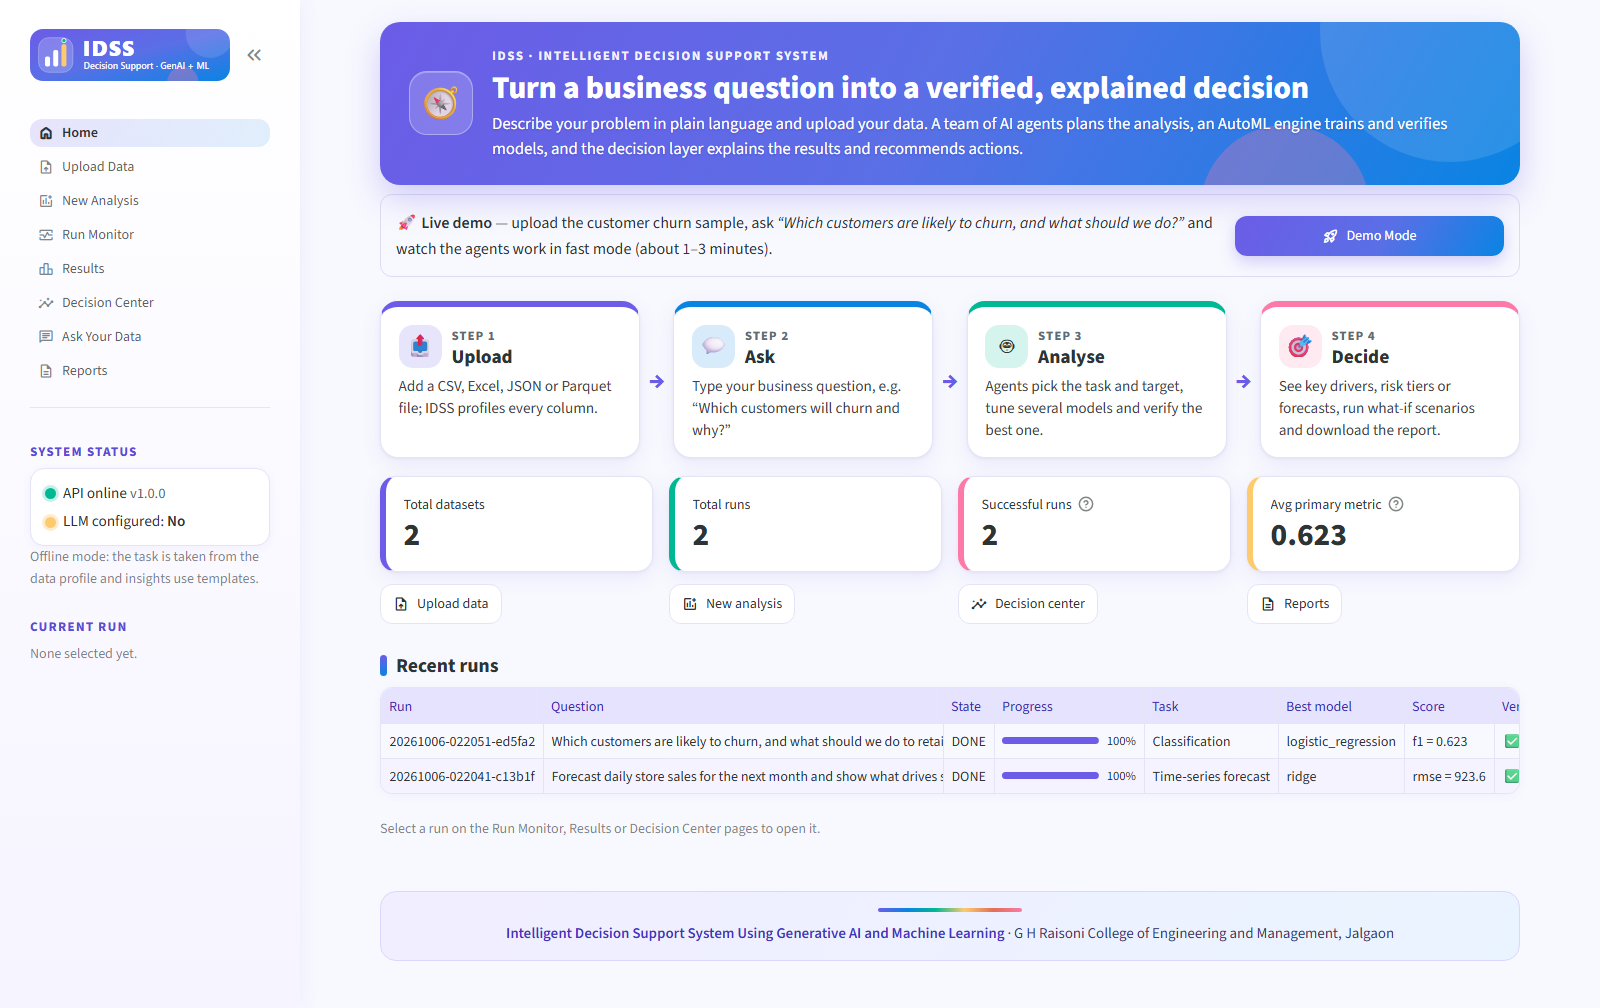
\includegraphics[width=\linewidth,height=7.3in,keepaspectratio]{figures/01_home.png}
  \caption{Home page: overview, Demo Mode, four-step flow, KPI strip and recent runs}\label{fig:5.1}
\end{figure}

\begin{figure}[htbp]
  \centering
  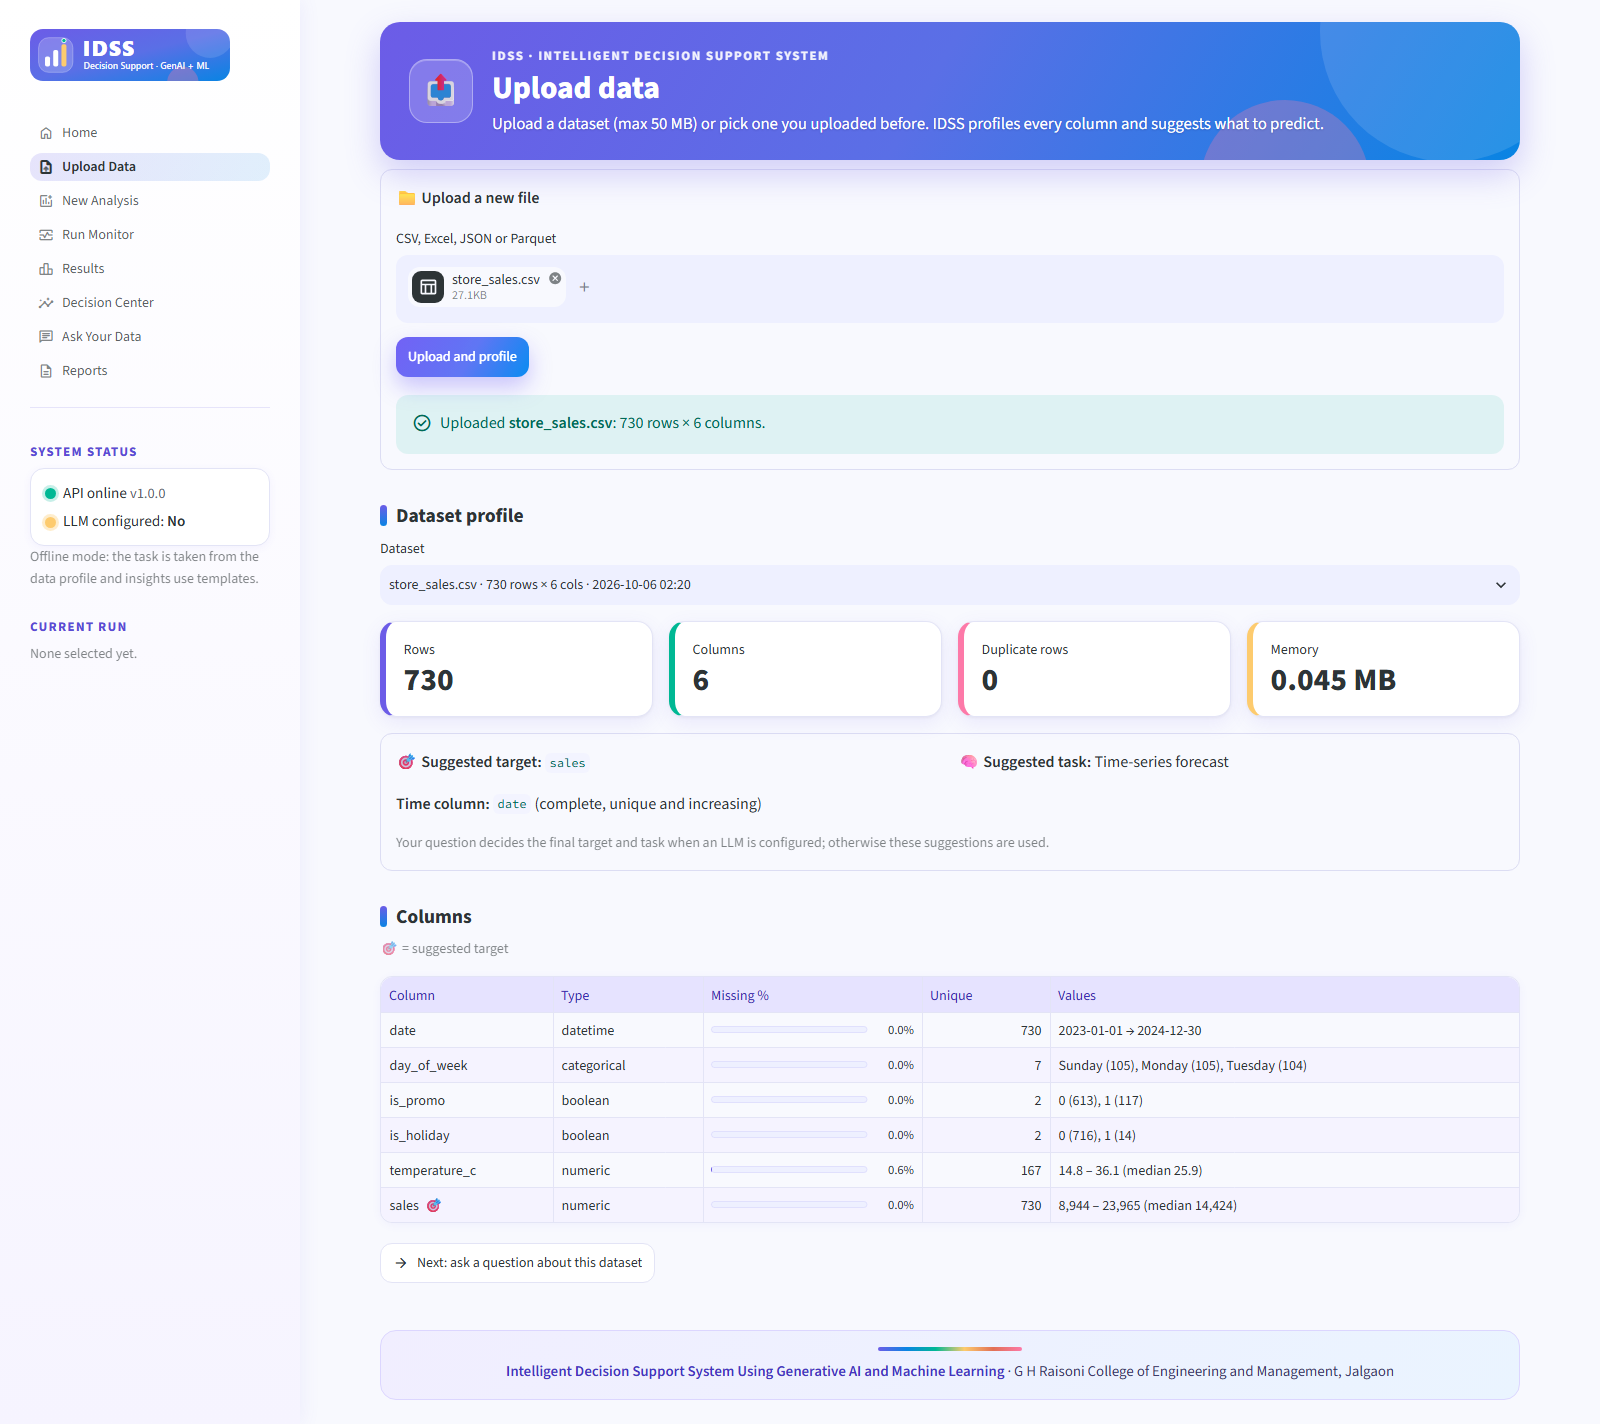
\includegraphics[width=\linewidth,height=7.3in,keepaspectratio]{figures/02_upload_profile.png}
  \caption{Upload Data page: profile of \code{store\_\allowbreak{}sales.csv} with types, missing values and suggested target and task}\label{fig:5.2}
\end{figure}

\begin{figure}[htbp]
  \centering
  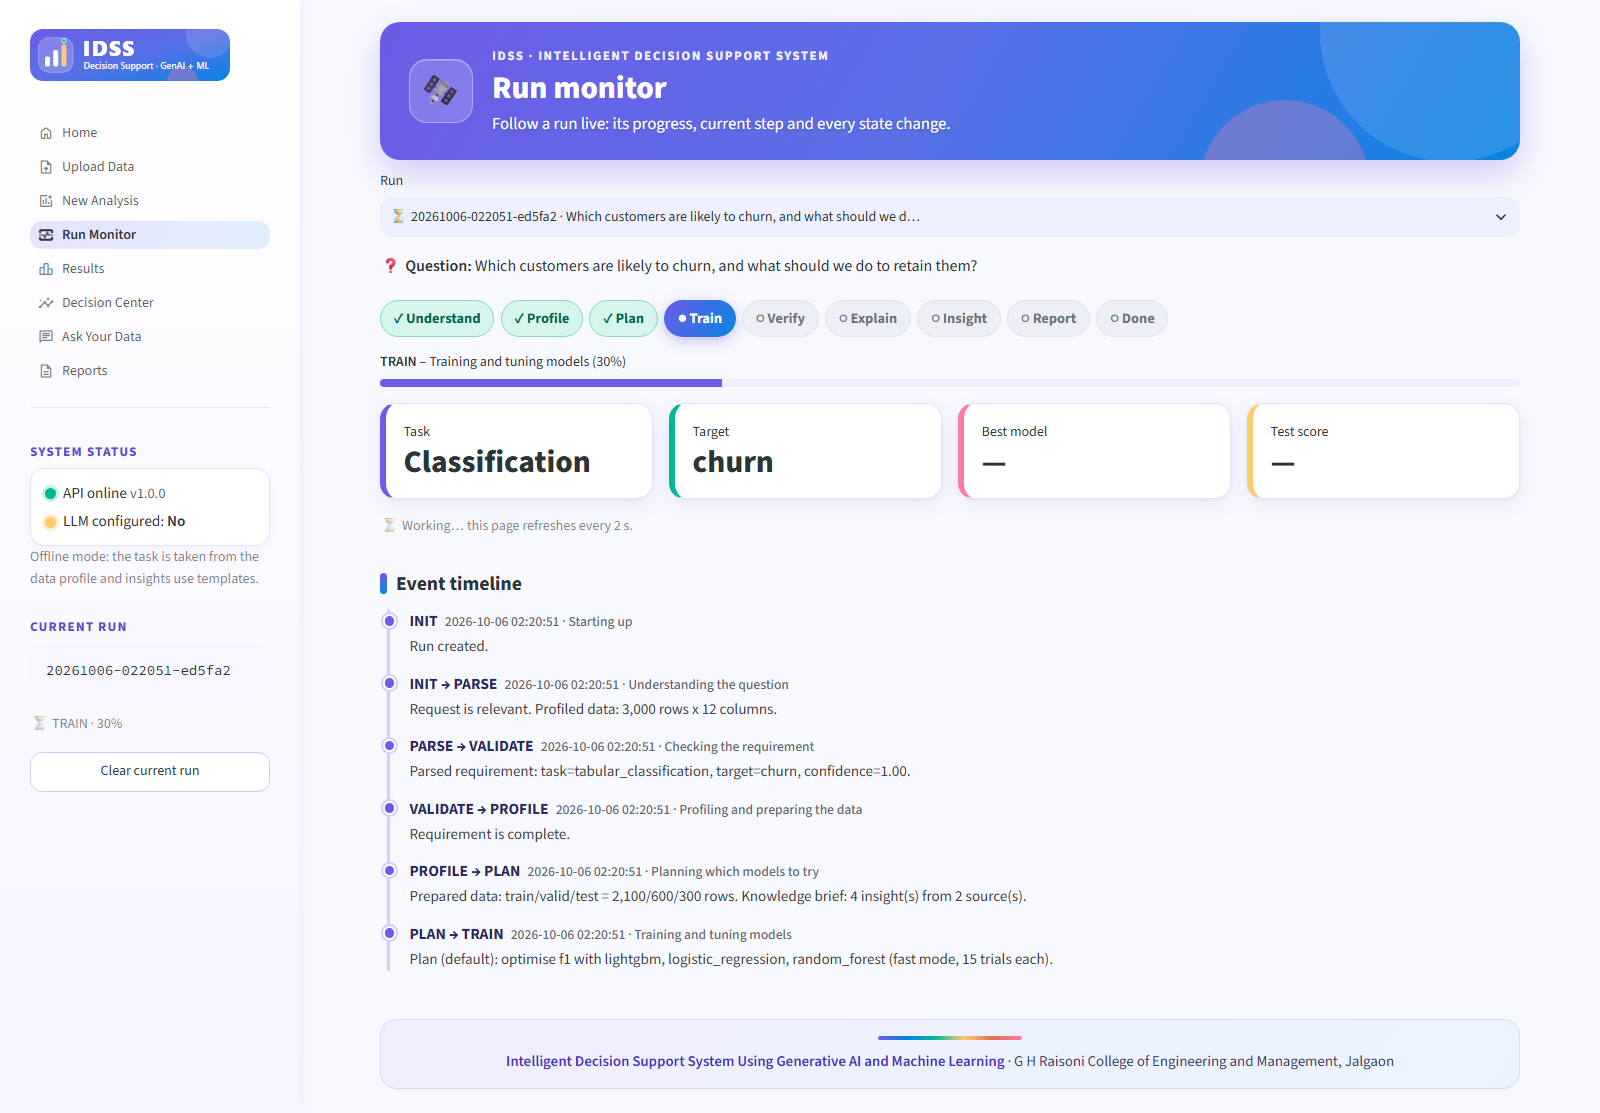
\includegraphics[width=\linewidth,height=7.3in,keepaspectratio]{figures/04_run_monitor.png}
  \caption{Run Monitor: pipeline stages, progress and event timeline of the churn run while it trains}\label{fig:5.3}
\end{figure}

\begin{figure}[htbp]
  \centering
  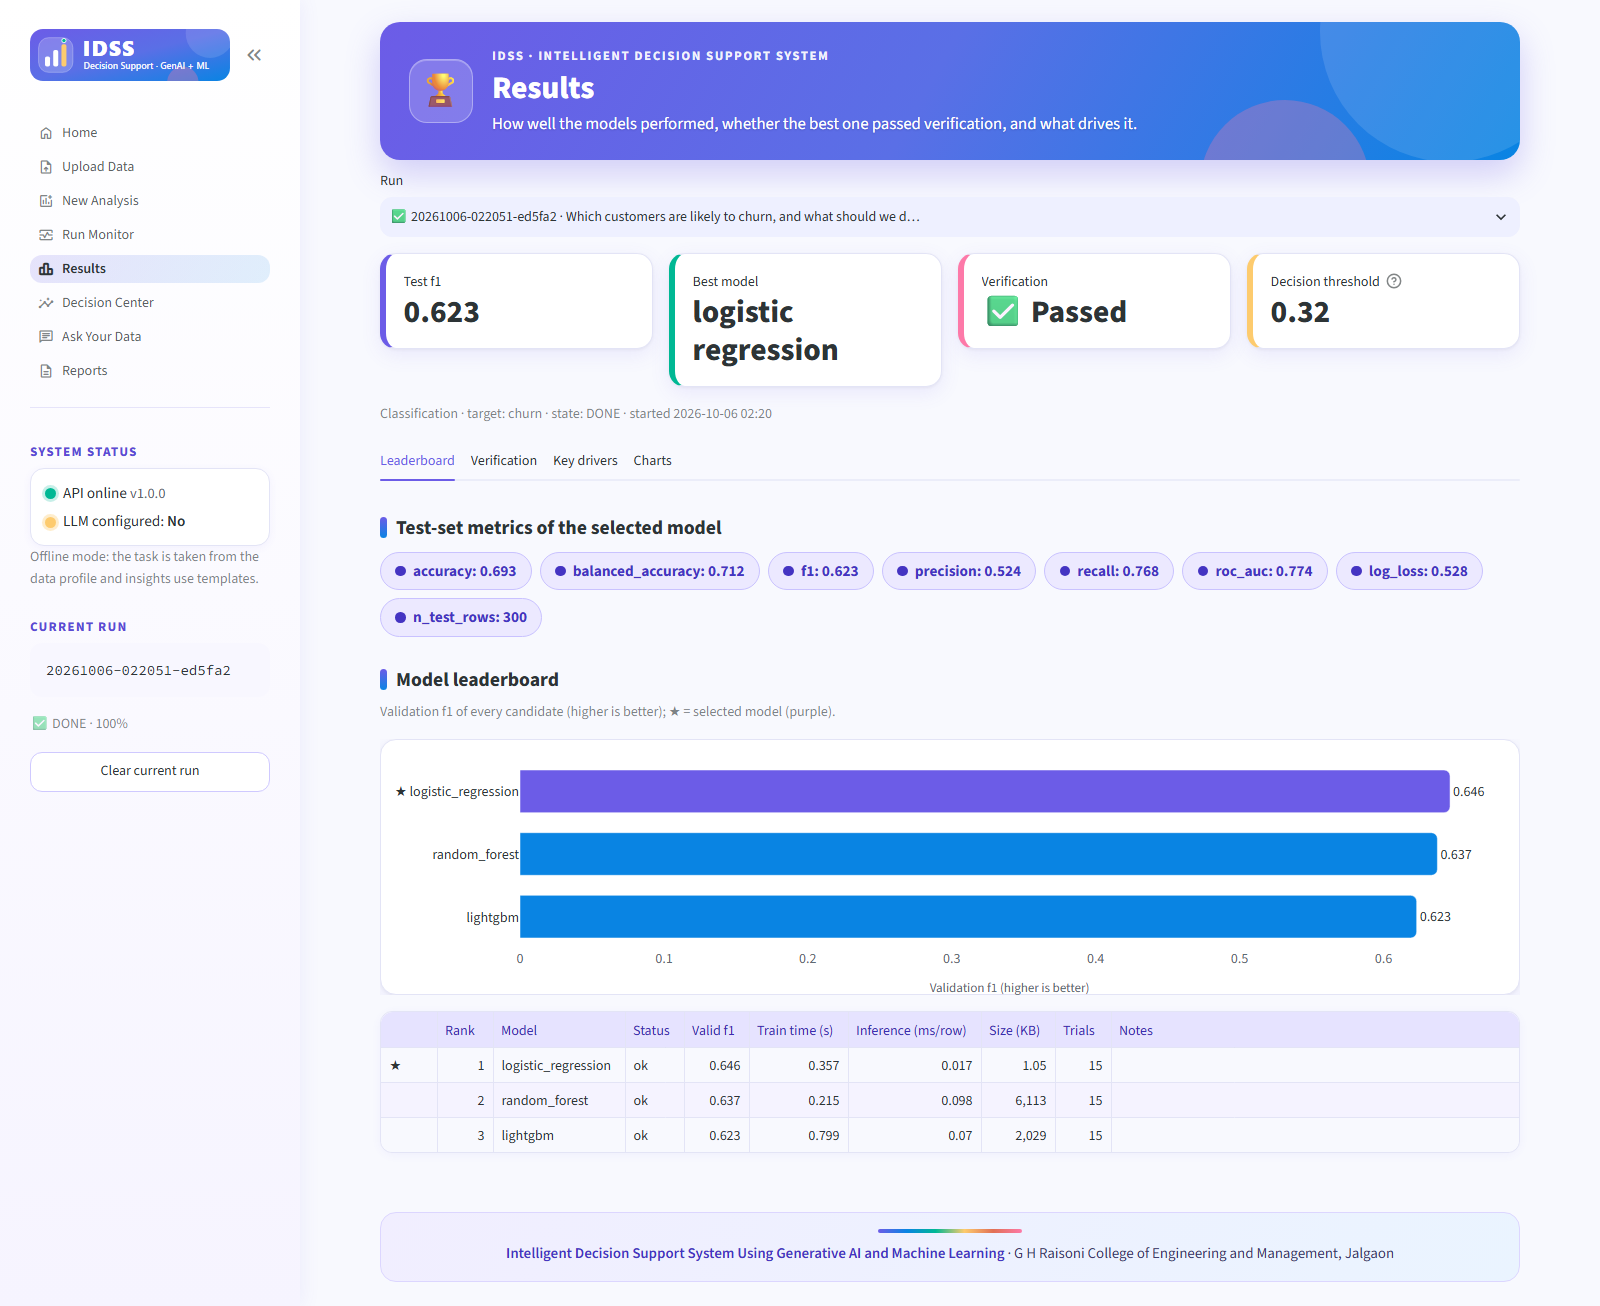
\includegraphics[width=\linewidth,height=7.3in,keepaspectratio]{figures/05_results.png}
  \caption{Results page: test metrics with leaderboard, verification, key-driver and chart tabs}\label{fig:5.4}
\end{figure}

\begin{figure}[htbp]
  \centering
  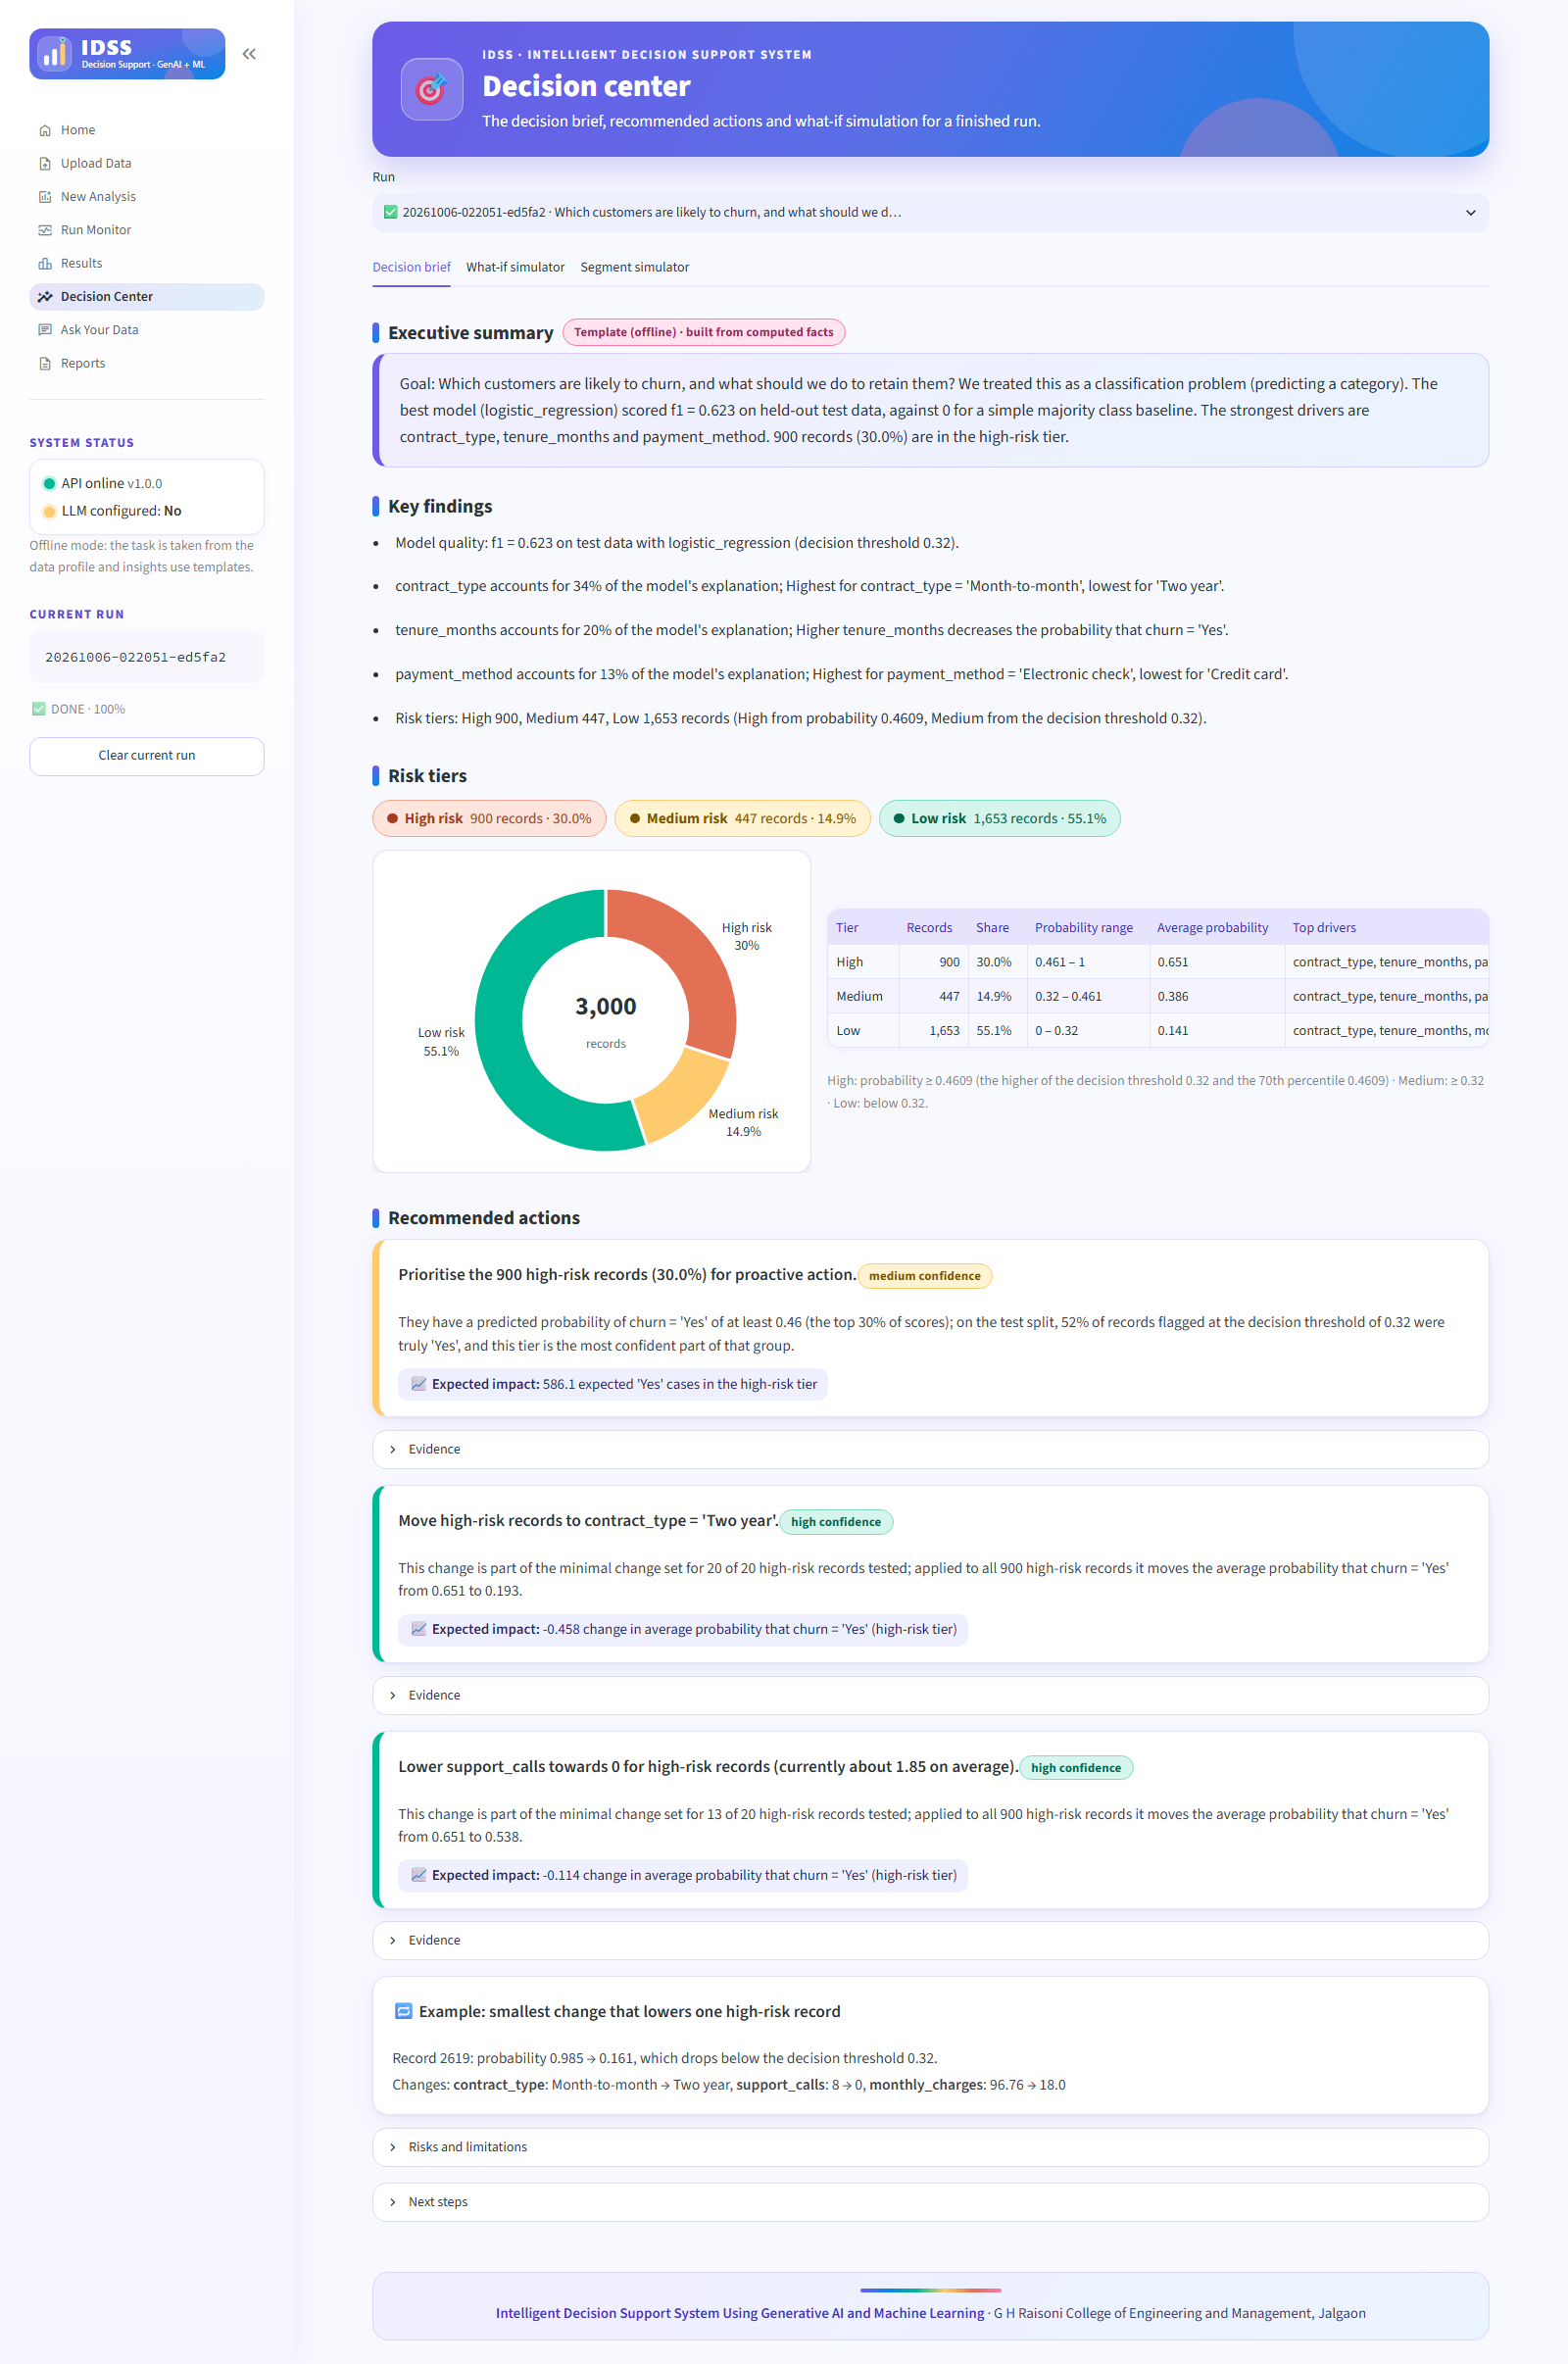
\includegraphics[width=\linewidth,height=7.3in,keepaspectratio]{figures/06_decision_center.png}
  \caption{Decision Center: executive summary, key findings, risk tiers and recommended actions for the churn run}\label{fig:5.5}
\end{figure}

\begin{figure}[htbp]
  \centering
  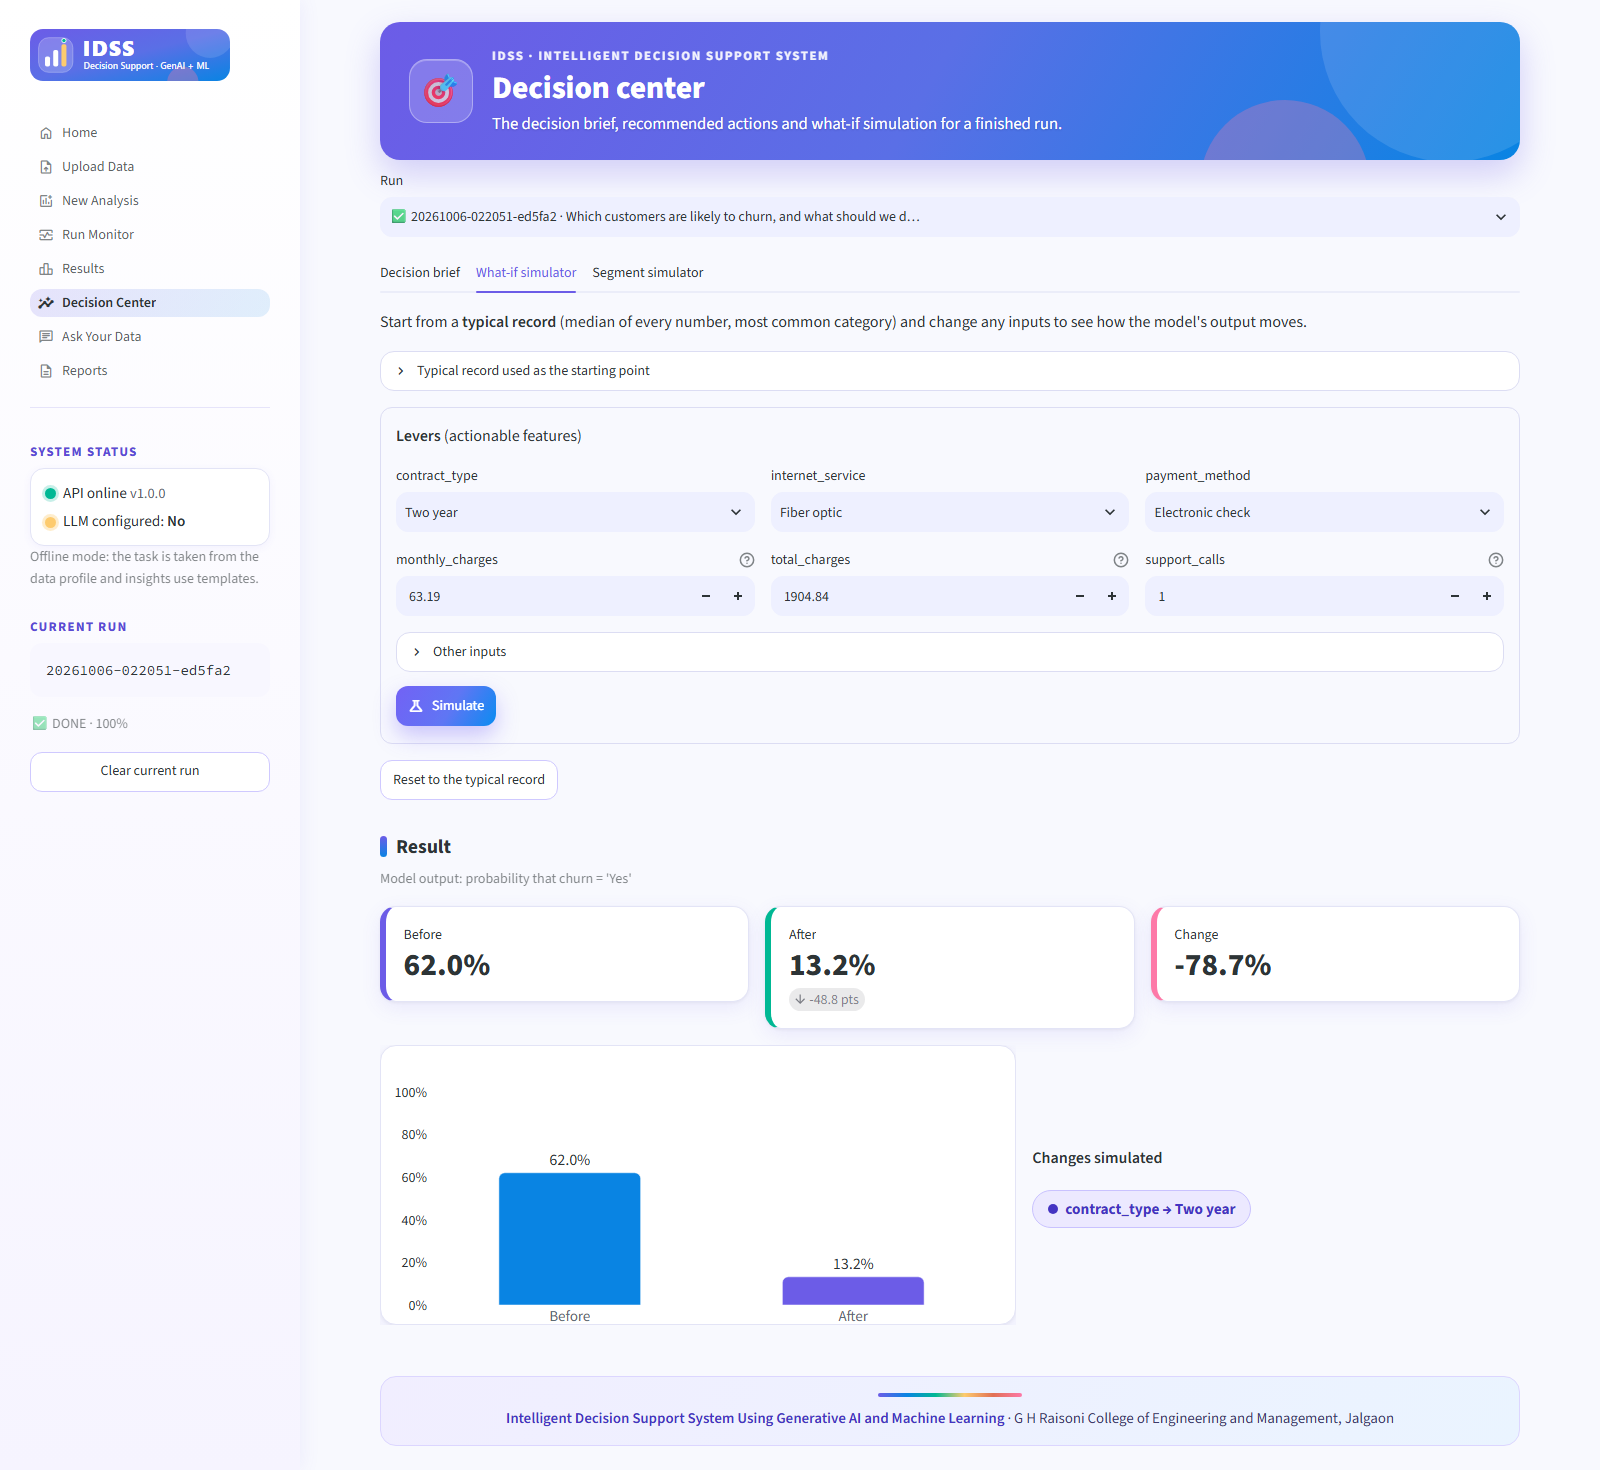
\includegraphics[width=\linewidth,height=7.3in,keepaspectratio]{figures/07_what_if.png}
  \caption{What-if simulator: a typical customer with \code{contract\_\allowbreak{}type} changed to ``Two year'', prediction before and after}\label{fig:5.6}
\end{figure}

\begin{figure}[htbp]
  \centering
  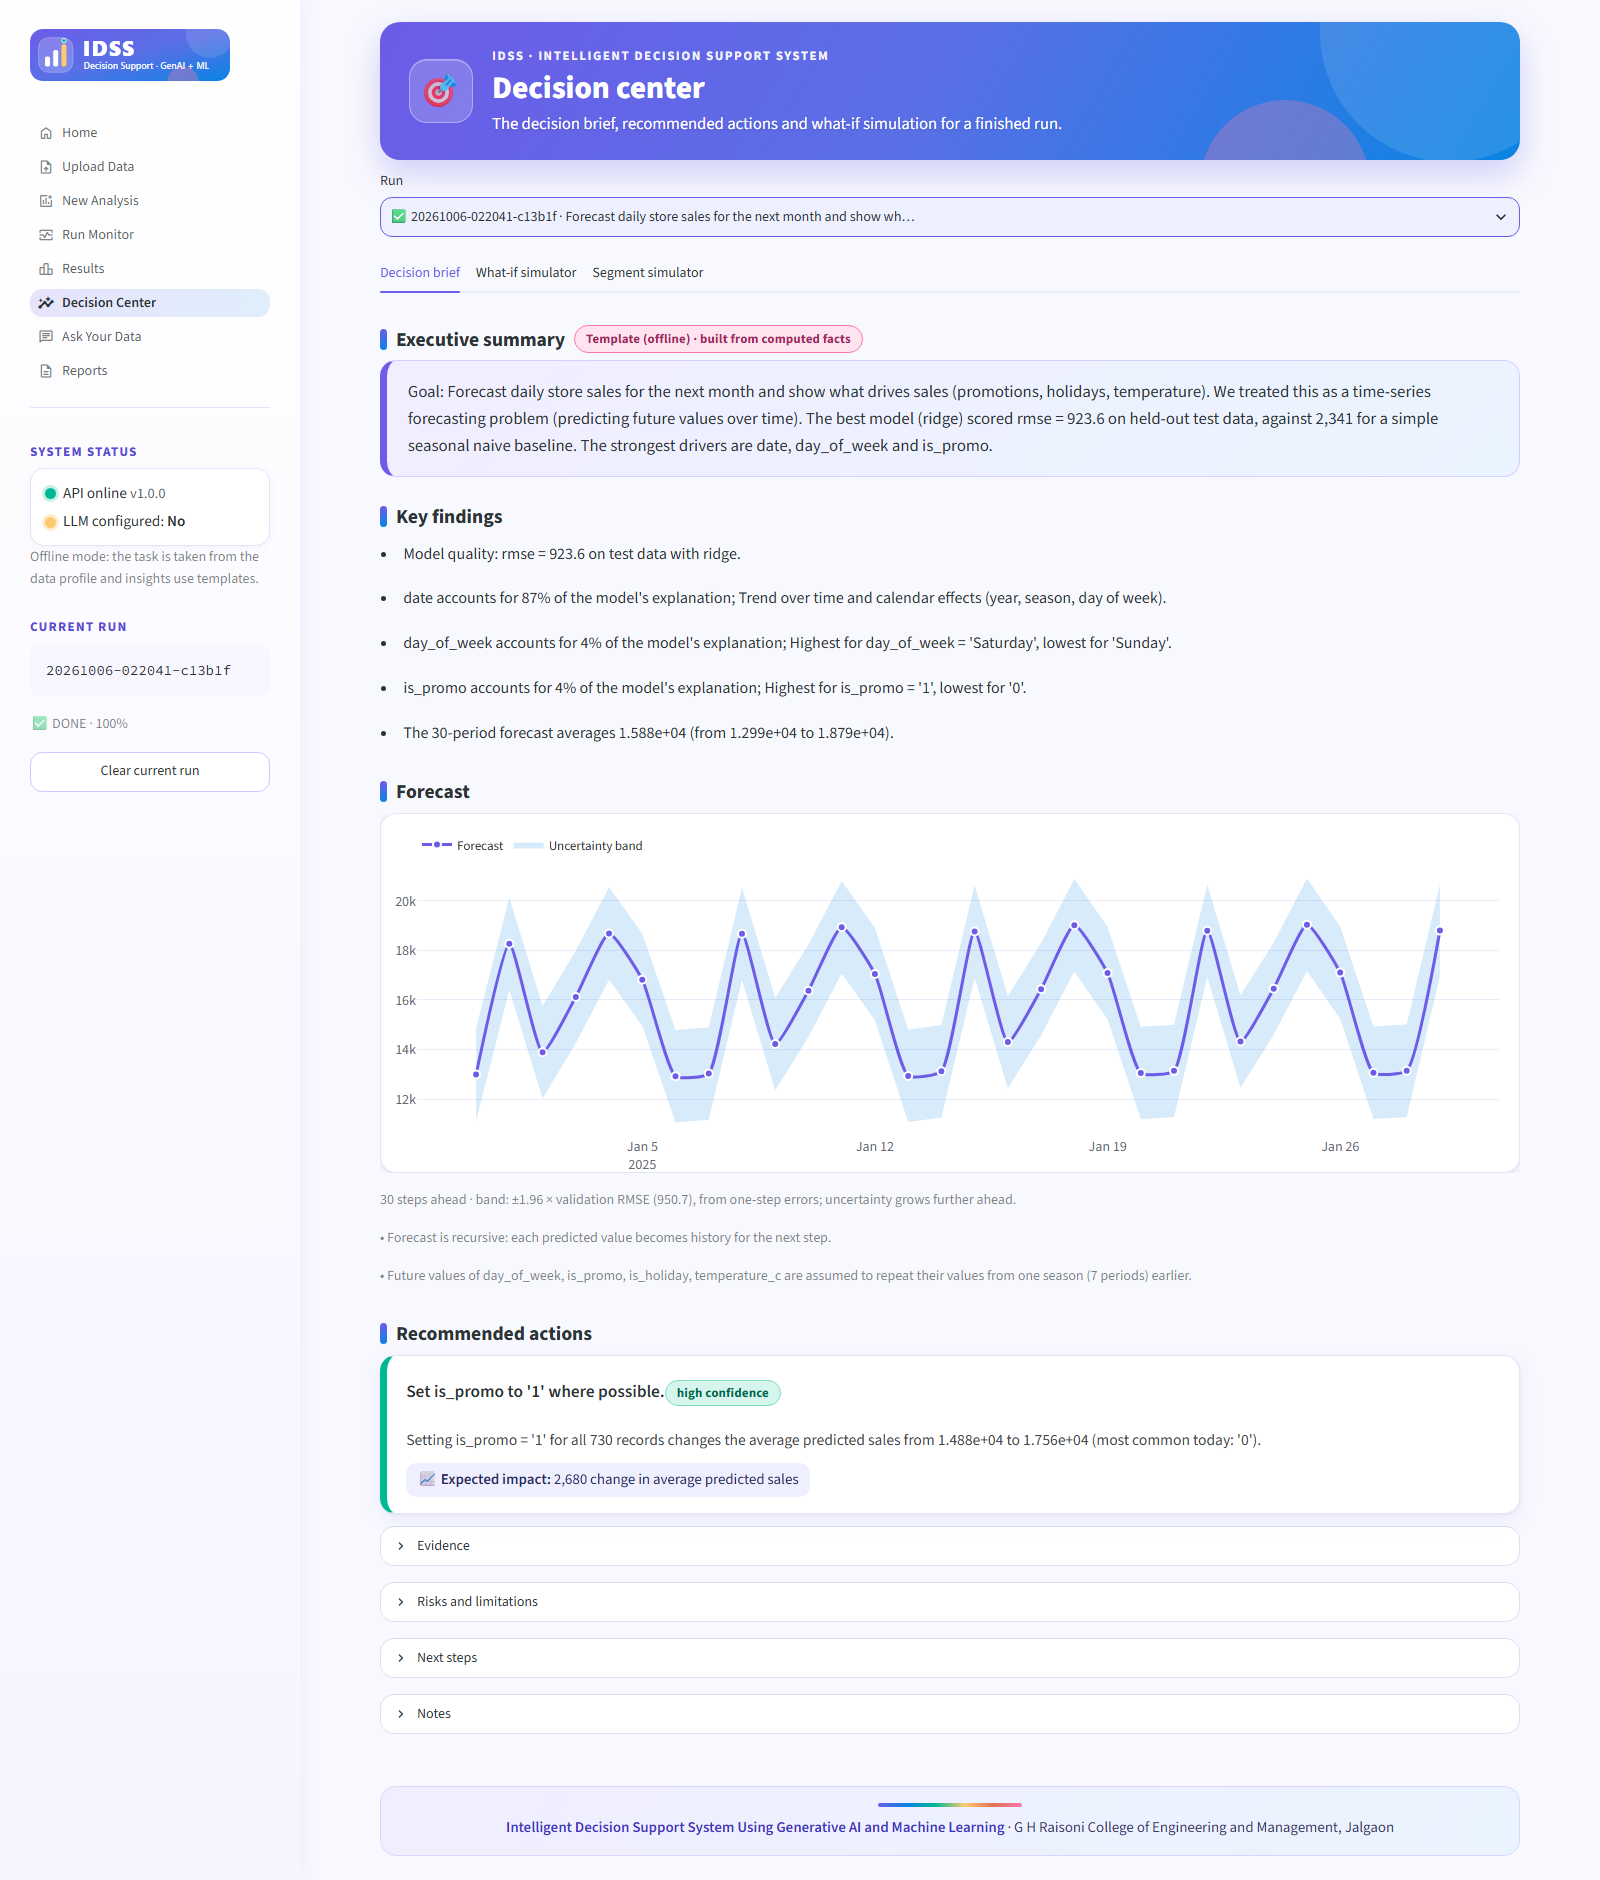
\includegraphics[width=\linewidth,height=7.3in,keepaspectratio]{figures/08_forecast.png}
  \caption{Decision Center for the store-sales run: forecast with its uncertainty band}\label{fig:5.7}
\end{figure}

\FloatBarrier
\section{Summary}\label{sec:5.6}

Eight algorithms capture the core logic: the state machine, requirement repair, the AutoML loop, threshold tuning, verification with re-planning, counterfactual search, the grounding check and the sandbox guard. Twelve modules implement them, each with a responsible member; short code extracts show how single use of the test split, contained failures, grounded numbers and sandboxed code are enforced; and the screenshots show the interface page by page.
